\documentclass[14pt,margin=0.5in,innermargin=0in,blockverticalspace=-0.1in]{tikzposter}
\geometry{paperwidth=841mm,paperheight=594mm}
\usepackage[utf8]{inputenc}
\usepackage{lmodern}
\usepackage{anyfontsize}
\usepackage{csquotes}
\usepackage{amsmath}
\usepackage{amsfonts}
\usepackage{amsthm}
\usepackage{amssymb}
\usepackage{mathrsfs}
\usepackage{graphicx}
\usepackage{adjustbox}
\usepackage{enumitem}
\usepackage{xcolor}
\usepackage[backend=biber,style=numeric,sorting=none]{biblatex}
\usepackage{durham-theme}
\usepackage{mwe} % for placeholder images

\addbibresource{references.bib}

% set theme parameters
\tikzposterlatexaffectionproofoff
\usetheme{DurhamTheme}
\usecolorstyle{DurhamStyle}

\usepackage[scaled]{helvet}
\renewcommand\familydefault{\sfdefault} 
\renewcommand{\vec}[1]{\bm{#1}}
\newcommand{\Tr}{\text{Tr}}
\usepackage[T1]{fontenc}

\title{Megapixel Image Generation with Step-unrolled Denoisng Autoencoders}
\author{\textbf{Alex F. McKinney}\textsuperscript{1},
\textbf{Dr. Chris G. Willcocks}\textsuperscript{1,2} 
}
\institute{\textsuperscript{1}Department of Computer Science, Durham University\\
            \textsuperscript{2}Project Supervisor
            }
\titlegraphic{
\includegraphics[width=0.16\linewidth]{durham-logo.png}}

% begin document
\begin{document}
\maketitle

\centering
\block{}
{
    \vspace{-2cm}
    \centering
    \begin{tikzfigure}[$1024 \times 1024$ samples from the FFHQ-1024 model. Each
        sample can be generated in $\approx 2$ seconds on a consumer-grade GPU.]
        \includegraphics[width=1.0\linewidth]{samples.png}
    \end{tikzfigure}
    \vspace{1cm}
    \begin{scope}[line width=\titlelinewidth,]
    \draw[color=colorThree!30!white,round cap-round cap]
    (\titleposleft,0)--(100,0);
    \end{scope}
}

\begin{columns}

    \column{0.32}
    \block{}{
        \vspace{-1cm}
        \begin{tikzfigure}[
                \textbf{Left:} Visualization of AR sampling. AR sampling
                proceeds one item at a time, resulting in the number of sampling steps
                being equal to the dimensionality of the input. For each prediction, a
                probability distribution over possible tokens is predicted and then
                sampled from. Each prediction can only make use of past context --
                indicated as a green position -- so not to violate the autoregressive
                property.
                \textbf{Right:} Visualization of NAR sampling. NAR
                sampling can sample an arbitrary number of items in parallel, including
                ones previously sampled, allowing for self-correction. It can freely use
                all context available to it, allowing for flexible inpainting and
                potentially better predictions.
            ]
            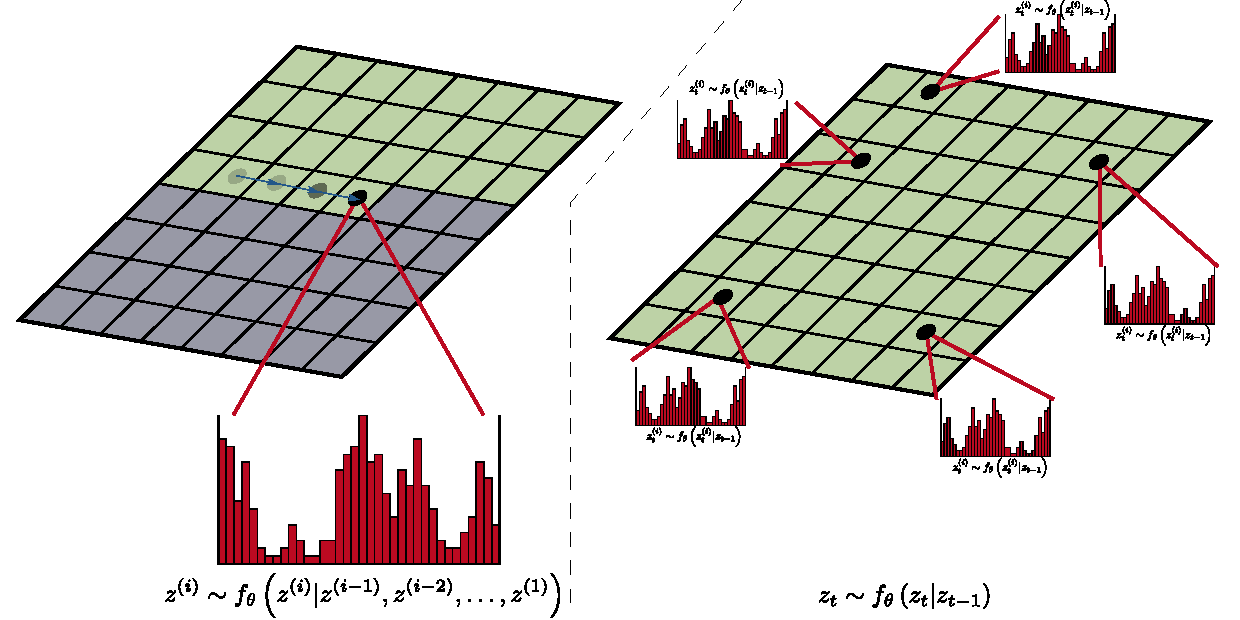
\includegraphics[width=1.1\linewidth]{AR-NAR.pdf}
        \end{tikzfigure}
    }
    
    \column{0.36}
    \block{}{
        \vspace{-1cm}
        \begin{tikzfigure}[$1024 \times 1024$ samples from the FFHQ-1024 model. Each
            sample can be generated in $\approx 2$ seconds on a consumer-grade GPU.]
            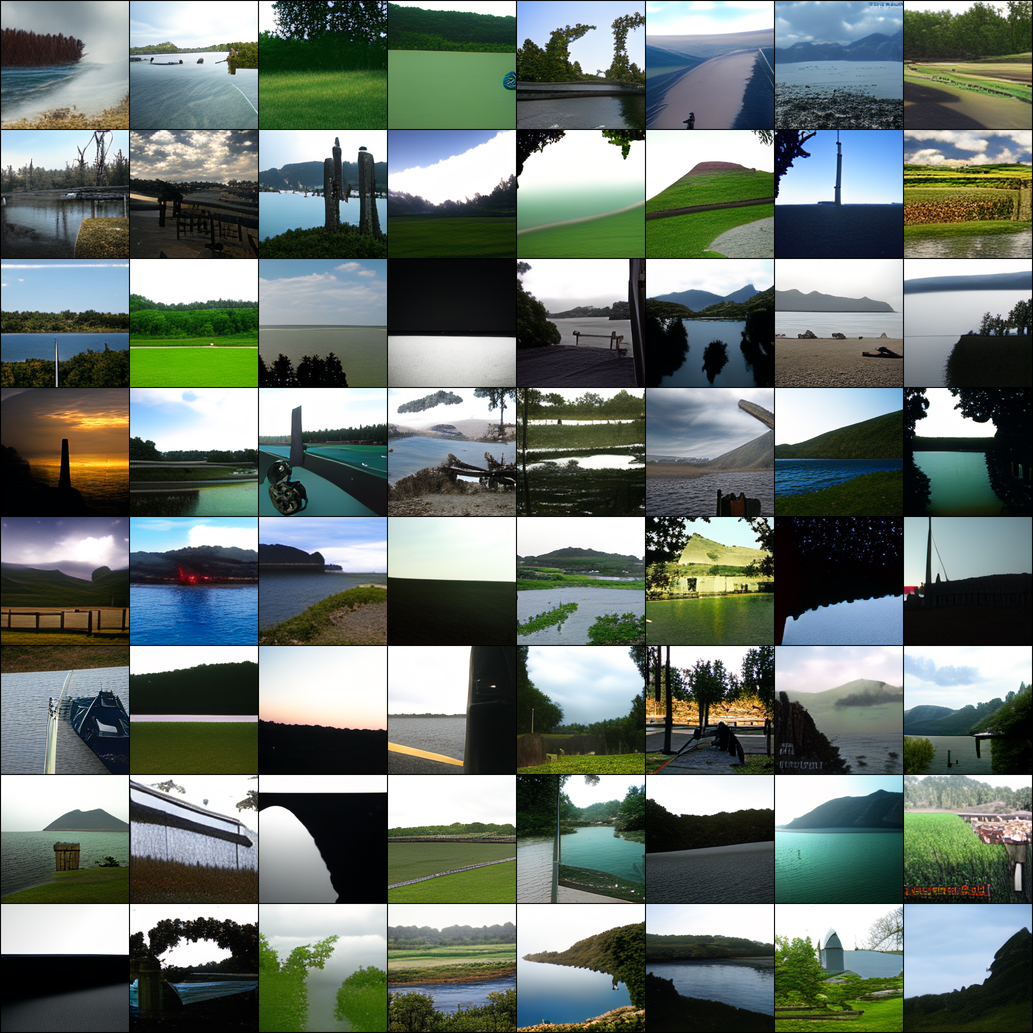
\includegraphics[width=0.49\linewidth]{imagenet-lakeside.png}
            \hfill
            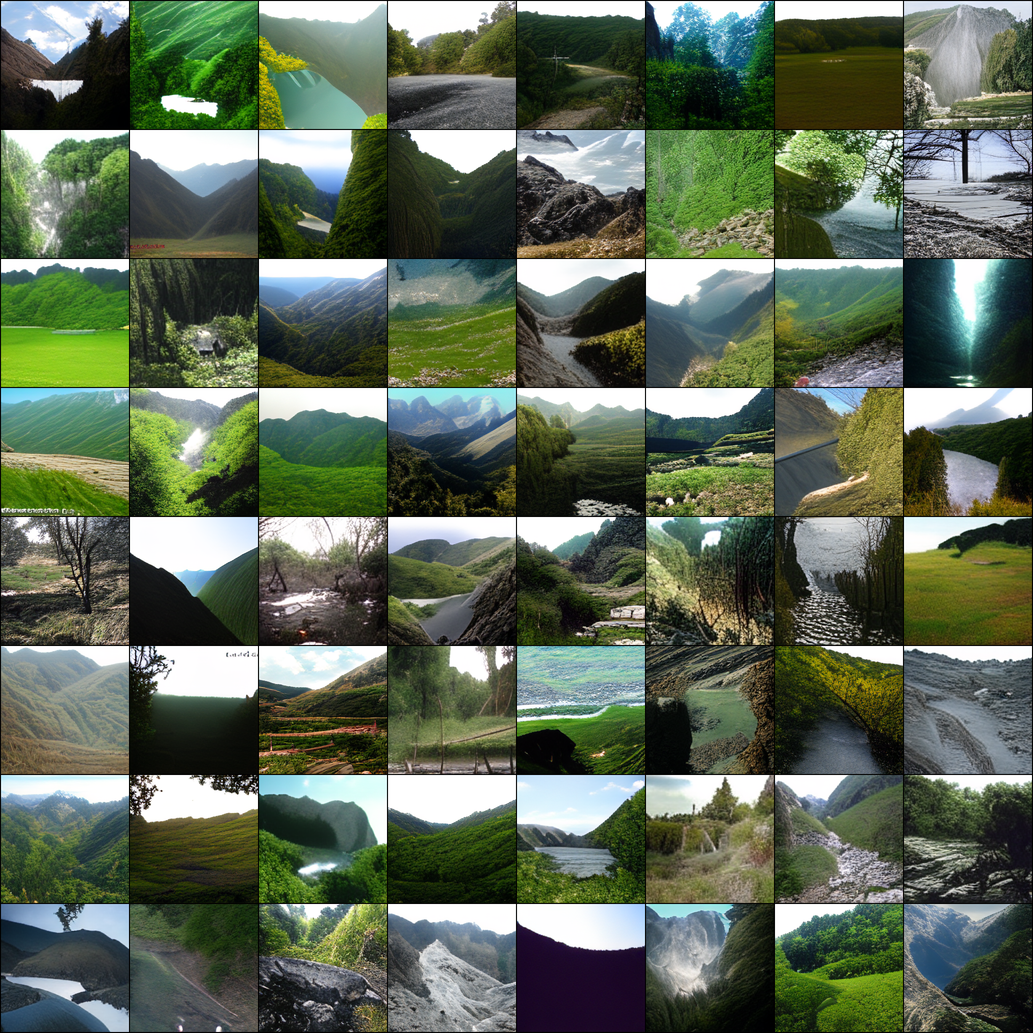
\includegraphics[width=0.49\linewidth]{imagenet-valley.png}
        \end{tikzfigure}
    }

    \column{0.32}
    \block{}{
        \vspace{-1cm}
        \begin{tikzfigure}[$1024 \times 1024$ samples from the FFHQ-1024 model. Each
            sample can be generated in $\approx 2$ seconds on a consumer-grade GPU.]
            \includegraphics[width=0.49\linewidth]{inpaint-rand.png}
            \hfill
            \includegraphics[width=0.49\linewidth]{inpaint-block.png}
        \end{tikzfigure}
    }

    \block{}{
        \vspace{-1em}
        \begin{footnotesize}
        \printbibliography[heading=none]
        \end{footnotesize}
    }
\end{columns}
\end{document}
